\documentclass[a4paper,ngerman]{scrartcl}

\usepackage{amsmath}
\usepackage{amsfonts}
\usepackage{amssymb}
\usepackage[utf8]{inputenc}
\usepackage{graphicx}
\usepackage[ngerman]{babel}
\usepackage{hyperref}
\usepackage{float}
\usepackage{caption}
\usepackage{subcaption}
\usepackage{multirow}  %for tables
\usepackage{icomma} % Handle german comma as decimal point in numbers
\usepackage{units,siunitx} % Write units with correct spacing
\usepackage{upgreek} % provide non-italic greek letters
\usepackage{url}
\usepackage{booktabs} % zu benutzen fuer \toprule und \bottomrule bei tabellen
%\usepackage{subfig}
\usepackage{extpfeil}

% Formatting of table & figure captions
\captionsetup{font={sf,footnotesize},labelfont=bf,skip=6pt}
\captionsetup[sub]{font={sf,footnotesize}} % setting for subcaptions
\sisetup{ locale = DE, % use "," as decimal point instead of "."
per-mode=fraction, % use fractions instead of ^{-1} when doing \si{... \per ...} 
exponent-product={\cdot},% used \cdot in front of 10^x
separate-uncertainty % give out uncertainty with \pm instead of in brackets
} 
\setlength{\abovecaptionskip}{6pt}
\setlength{\belowcaptionskip}{0pt}

\title{Black Lipid Membrane\\ Verbesserung}
\date{\today}
\author{Michel Rausch, Michael Eliachevitch}

\begin{document}

\maketitle
\tableofcontents
\newpage

\section{Vorbereitung}

\subsection{Ionentransport}

Es existieren verschiedene Modelle, die beschreiben, wie Gramicidin A in die Zellmembran integriert wird, welche in Abbildung \ref{fig:wirkmechanismus} aufgelistet sind. Auf die chemischen Grundlagen der Modelle wird nicht im Detail eingegangen.
  
%Punkt B neu schreiben, alle Punkte etwas ausformulieren.

\begin{figure}[tbh!]
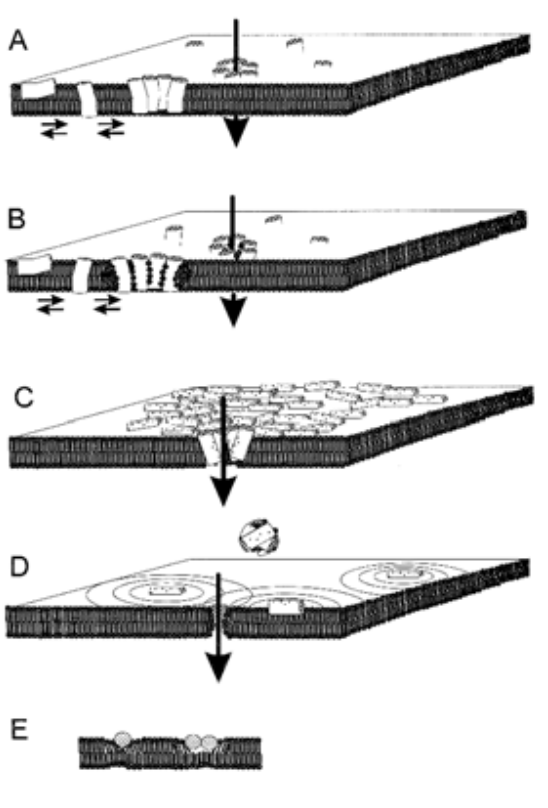
\includegraphics[width=0.5\textwidth]{abbildungen/wirkmechanismus.png}
\caption{\textbf{Verschiedene Modelle zur Erklärung der Zerstörung einer Bakterienzelle mittels Peptid-Antibiotika [\ref{ref:mappe}].}\\
\textbf{A: Barrel Stave model,} 
Hydrophobe, helixförmige Monomere bilden Poren in der Zellmembran.
\textbf{B: Toroidial Wormhole model,}  
Porenformation in Anwesenheit phosphatidylethanolaminer, oder phosphatidylseriner Membranen. 
\textbf{C: Carpet model}  
Teppich-(engl. carpet-)ähnliche Anlagerung auf Membran.
\textbf{D:  Detergent similar model,}
Bi- und Mizellen bilden Flächen auf der Membran, durch deren Amphiphilie wird die Membran durchlässig.
\textbf{E:  In-plane diffusion model,}
Verdünnung der Lipidschicht.
}
\label{fig:wirkmechanismus}
\end{figure}


\subsection{Einzelkanalentstehung}

%Folgender Teil besser formuliert
Nur Dimere des Gramicidin A führen zu einer Bildung von Ionenkanälen. 
Ist die Rate der Bildung der Dimere gleich der Rate ihrer Vernichtung, spricht man von einem Gleichgewicht.
Ohne äußere Einwirkung bleibt die Zahl der Kanäle also etwa gleich.
Die Bildung und Zerstörung sind zufällige Ereignisse, daher kommt es zu einer variierenden Anzahl an Poren in der Membran und somit zu einer Fluktuation der Leitfähigkeit. 
Bei einer geringen Konzentration sind nur einzelne Kanäle vorhanden, daher ist die Quantisierung des Stromes $I_M$ deutlich erkennbar.

Die Dimerasation kann durch die Gleichung,

\begin{equation}
G_1 + G_1 	\xtofrom[k_d]{k_r} G_2 ,
\end{equation}

beschrieben werden. $k_d$ ist hier die Rate der Dissoziation und $k_r$ die der Entstehung der Dimere, $G_1$ entspricht den Monomeren, $G_2$ den Dimeren. Die Dissoziation folgt einem exponentiellem Zerfallsgesetz, die der Entstehungsreaktion ist linear zum Quadrat der Konzentration. Aus dem Verlauf des Stromes über die Zeit lässt sich die Zerfallsrate bestimmen.



\section{Auswertung}


\subsection{Aufgabe 3: Messung multipler Ionenkanäle}

Die Stammlösung betrug $\SI{0.1}{\milli \gram \per \milli \litre}$ und wurde mit Wasser zu $\SI{4}{\nano \gram \per \milli \litre}$ verdünnt.
Die Spritze wurde vollständig entleert. 
Damit befanden sich \SI{1}{\milli \litre} der Gramicidin A-Lösung in der Küvette.
Da das Volumen der Salzlösung in der Küvette nicht bekannt war, konnte die entgültige Konzentration des Gramicidin A nicht bestimmt werden.
Diese ist zum Auswerten des Versuchs nicht unbedingt notwendig, da qualitative Effekte betrachtet werden sollen.
Es ist vor allem wichtig, das die Konzentration hoch genug ist, um den gewünschten Effekt zu erzielen, jedoch nicht zu hoch, um die Messung unmöglich zu machen.
Unter diesen Bedingungen war es noch schwieriger eine stabile Lipidschicht aufzubauen, als bei den Aufgabe zuvor.
Sie platzte meist nach kurzer Zeit, insbesondere nach Anlegen einer Spannung, sodass die Messung nur in einem Intervall von einer Minute erfolgen konnte.
Die Konzentration war hoch genug, dass sich mehrere Kanäle geöffnet haben und eine Einkanaluntersuchung nicht mehr möglich war.




\clearpage
\section{Quellen}
\begin{enumerate}
\item Vorbereitungsmappe \label{ref:mappe}
\item http://www.chemie.de \label{ref:chemie.de}
\item http://www.wolframalpha.com \label{ref:wolfram}
\end{enumerate}




\end{document}
